
\documentclass{jtetiproposalskripsi}

%-----------------------------------------------------------------
%Disini awal masukan untuk data proposal tugas akhir
%-----------------------------------------------------------------
\titleind{PERANCANGAN SISTEM INFORMASI REKAM DATA MEDIS DI KLINIK KASIH IBU KALISAT}
\fullname{DIAH SILFIANA}

\idnum{1200631011}

\approvaldate{14 Januari 2015}

\degree{Diploma Manajemen Informatika}

\yearsubmit{2015}

\program{Manajemen Informatika}

\headprogram{Sarjiya, S.T., M.T., Ph.D.}

\dept{}

\firstsupervisor{Triawan Adi Cahyanto,M.Kom}
\firstnip{12 03 719}

\secondsupervisor{Bagus Setya Rintyarna,S.T,M.Kom}
\secondnip{09 03 521}


%-----------------------------------------------------------------
%Disini akhir masukan untuk data proposal skripsi
%-----------------------------------------------------------------

\begin{document}

\cover

\approvalpage

%-----------------------------------------------------------------
%Disini akhir masukan untuk muka skripsi
%-----------------------------------------------------------------

%-----------------------------------------------------------------
%Disini awal masukan Intisari
%-----------------------------------------------------------------
\begin{abstractind}
Klinik Kasih Ibu merupakan suatu Organiasasi yang bergerak dibidang pelayanan kesehatan masyarakat. Pada Klinik Kasih Ibu ini dalam memberikan pelayanan kepada pasien dan mendata obat masuk masih dilakukan dengan cara manual atau belum terkomputerisasi. Media penyimpanan data pasien menggunakan media kertas sehingga mengakibatkan pencarian data dilakukan dengan cara menelusuri arsip-arsip yang dapat menyita waktu serta setiap entitas belum terintegrasi sehingga menyebabkan informasi yang dihasilkan lambat, kurang akurat dan tidak relevan. 

Untuk mendukung metode pengembangan Sistem Informasi Rekam Data Medis yang dibuat sekarang penulis menggunakan metode waterfall. Serta teknik pengumpulan data dengan metode. Penelitian dengan cara observasi, wawancara dan studi pustaka. Implementasi program yang digunakan komputer pada sistem rekam data medis ini menggunakan bahasa pemrograman Visual Basic 6.0 dengan database MySQL yang menyediakan fasilitas untuk mempermudah proses pembuatan sistem informasi dan implementasi produk. 

Sistem Informasi yang dibuat dapat mengatasi permasalahan-permasalahan yang ada diKlinik Kasih Ibu. Media Penyimpanan, pengolahan data pasien, rekam medis, dan obat sudah dapat terintegrasi dengan baik sehingga karyawan dan dokter dapat lebih mudah dan cepat dalam melayani pasien yang melakukan pengobatan.

\begin{flushleft}

\textbf{Kata Kunci} : \textit{Klinik Kasih Ibu, Sistem Informasi Rekam Data Medis}
\end{flushleft}

\bigskip

\end{abstractind}
%-----------------------------------------------------------------
%Disini akhir masukan Intisari
%-----------------------------------------------------------------

\tableofcontents
\addcontentsline{toc}{chapter}{DAFTAR ISI}
\selectlanguage{bahasa}\clearpage\pagenumbering{arabic}\setcounter{page}{1}

%-----------------------------------------------------------------
%Disini awal masukan untuk Bab
%-----------------------------------------------------------------
\chapter{PENDAHULUAN}

\section{Latar Belakang Masalah}
Dalam era globalisasi saat ini, ilmu pengetahuan dan teknologi berkembang begitu pesat, khususnya teknologi informasi. Kebutuhan manusia akan segala sesuatu dituntut lebih efisien,contohnya sangat jelas terasa dari perkembangan teknologi informasi tersebut, pekerjaan yang semula masih banyak menggunakan sistem manual pada saat ini sudah mulai berkurang, karena mulai beralih ke sistem yang sudah terkomputerisasi.Karena dengan proses yang sudah terkomputerisasi pekerjaan apapun akan lebih mudah dilakukan. Dalam proses perkembangan kebutuhan data dan informasi yang semakin lama berkembang, telah mendorong penanganan data dan informasi yang lebih baik agar setiap unsur tersebut dapat dilaksanakan dengan optimal.Penerapan suatu sistem data dan informasi pada dasarnya tidak terlepas dari penggunaan komputer itu sendiri. Agar lebih mudah menginputkan data pada sistem dalam hal ini aplikasi tentang klinik,sistem ini dirancang agar proses registrasi dan penanganan terhadap pasien di klinik tersebut agar segera di tangani penyakitnya secara sigap tanpa harus mendata mereka secara manual. Dengan adanya sistem yang baru ini dapat memberikan solusi bagaimana cara mendapatkan pelayanan dengan proses yang cepat namun dengan harga yang terjangkau. Menyadari banyaknya klinik yang sudah ada bergerak dibidang yang sama, maka klinik tersebut harus melakukan terobosan – terobosan baru demi meningkatkan kualitas dan berusaha menarik minat para pasien sehingga klinik tersebut makin mendapat tempat di hati masyarakat. Berdasarkan latar belakang diatas, maka dianggap perlu untuk membuat sistem yang akan dapat membantu mempermudah pengelolaan data pasien, serta mempercepat penanganan daripada pasien tersebut, sehingga penulis mengambil judul : \textit{Perancangan Sistem Informasi Rekam Data Medis di Klinik Kasih Ibu Kalisat}

\section{Rumusan Masalah}
Adapun rumusan masalah dalam penelitian ini adalah sebagai berikut :
\begin{enumerate}
\item Bagaimana menganalisis dan Perancangan Sistem Informasi Rekam Data Medis di Klinik Kasih Ibu Kalisat secara terkomputerisasi.
\item Bagaimana membangun Perancangan Sistem Informasi Rekam Data Medis di Klinik Kasih Ibu Kalisat agar mudah digunakan oleh petugas?
\item Software apa dan database apa yang digunakan untuk  membangun Perancangan Sistem Informasi Rekam Data Medis di Klinik Kasih Ibu Kalisat?
\end{enumerate}

\section{Batasan Masalah}
Batasan yang diperlukan untuk mengetahui ruang lingkup pembahasan suatu masalah, mengingat begitu luasnya permasalahan yang ada serta keterbatasan pengetahuan yang dimiliki. Penulis membatasi ruang lingkup yang akan dibahas yaitu:
\begin{enumerate}
\item Pengguna dari sistem ini adalah seorang admin. Disini admin bertugas untuk entry data pasien, dokter, hasil pemeriksaan dan pembayaran. 
\item Teknologi pemrograman yang digunakan untuk membuat dan membangun aplikasi adalah Visual Basic 6.0
\item Untuk mengelola database digunakan oracle 10g 
\item Sistem ini terdiri dari pendataan pasien, dokter, hasil pemeriksaan dan pembayaran pasien tersebut.
\end{enumerate}

\section{Tujuan Penelitian}
Adapun tujuan dari sistem informasi klinik ini adalah sebagai berikut:
\begin{enumerate}
\item Merubah sistem informasi yang bersifat manual menjadi sebuah sistem yang berbasis komputer
\item Mempermudah petugas dalam melakukan pendataan pasien.

\end{enumerate}

\section{Manfaat Penelitian}
Adapun manfaat dari penelitian ini yakni :
\begin{enumerate}
\item Hasil penelitian ini dapat dijadikan bahan referensi bagi peneliti selanjutnya.
\item Mempermudah petugas dalam melakukan pendataan pasien melalui aplikasi rekam medis.
\item Penelitian ini dapat menambah wawasan dan pengetahuan bagi penulis tentang perancangan Perancangan Sistem Informasi Rekam Data Medis menggunakan Visual Basic sesuai tuntutan zaman.
\end{enumerate}

\section{Metodelogi Penelitian}
Metode yang diterapkan dalam pencarian data meliputi dua macam metode yakni :
\begin{enumerate}
\item Metode Observasi Secara Langsung Metode observasi ini dilakukan dengan melihat proses kerja yang terjadi di lapangan yakni di lingkungan kerja Klinik Kasih Ibu Kalisat .
\item Metode Wawancara Metode ini digunakan untuk mengetahui permasalahan maupun proses kerja yang terjadi di instansi. Dengan narasumber yang berkompeten sehingga didapatkan data-data yang akurat. Hal ini dapat mempermudah melakukan proses analisis permasalahan.
\end{enumerate}

\section{Sistematika Penulisan}
Uraian singkat mengenai struktur penulisan pada masing-masing bab adalah sebagai berikut:

\begin{quote}
\textbf {BAB I PENDAHULUAN}
Membahas Latar Belakang Masalah, Identifikasi Masalah, Batasan Masalah, Tujuan Penelitian, Metodelogi Penelitian serta Sistematika Penulisan.

\textbf {BAB II LANDASAN TEORI}
Memaparkan teori-teori yang didapat dari sumber-sumber yang relevan untuk digunakan sebagai panduan dalam penelitian serta penyusunan laporan tugas akhir.

\textbf {BAB III METODOLOGI PENELITIAN}
Berisi tentang perancangan sistem serta komponen-komponen pemodelan sistem yang digunakan.

\textbf {BAB IV PENUTUP}
Mengemukakan kesimpulan yang diambil dari hasil penelitian dan perancangan sistem, serta saran-saran untuk pengembangan selanjutnya, agar dapat dilakukan perbaikan-perbaikan di masa yang akan datang.

\end{quote}

%-------------------------------------------------------------------------------
\chapter{LANDASAN TEORI}                

\section{Pengertian Sistem Informasi}
Sistem Informasi (SI) adalah kombinasi dari teknologi informasi dan aktivitas orang yang menggunakan teknologi itu untuk mendukung operasi dan manajemen. Dalam arti yang sangat luas, istilah sistem informasi yang sering digunakan merujuk kepada interaksi antara orang, proses algoritmik, data, dan teknologi. Dalam pengertian ini, istilah ini digunakan untuk merujuk tidak hanya pada penggunaan organisasi teknologi informasi dan komunikasi (TIK), tetapi juga untuk cara di mana orang berinteraksi dengan teknologi ini dalam mendukung proses bisnis.

Dengan demikian, sistem informasi antar-berhubungan dengan sistem data di satu sisi dan sistem aktivitas di sisi lain. Sistem informasi adalah suatu bentuk komunikasi sistem di mana data yang mewakili dan diproses sebagai bentuk dari memori sosial. Sistem informasi juga dapat dianggap sebagai bahasa semi formal yang mendukung manusia dalam pengambilan keputusan dan tindakan.

\section{Pengertian Klinik}
Klinik adalah fasilitas pelayanan kesehatan yang menyelenggarakan pelayanan kesehatan perorangan yang menyediakan pelayanan medis dasar dan/ sepesialistik, diselenggarakan oleh lebih dari satu jenis tenaga kesehatan (perawat atau bidan) dan pemimpin oleh seorang tenaga medis (dokter, dokter spesialis, dokter gigi atau dokter gigi spesialis).

\section{Bahasa Pemrograman Visual Basic}
Microsoft Visual Basic .NET adalah sebuah alat untuk mengembangkan dan membangun aplikasi yang bergerak di atas sistem .NET Framework, dengan menggunakan bahasaBASIC. Dengan menggunakan alat ini, para programmer dapat membangun aplikasi Windows Forms, Aplikasi web berbasis ASP.NET, dan juga aplikasi command-line.  Bahasa Visual Basic .NET sendiri menganut paradigma bahasa pemrograman berorientasi objek yang dapat dilihat sebagai evolusi dari Microsoft Visual Basic versi sebelumnya yang diimplementasikan di atas .NET Framework. Peluncurannya mengundang kontroversi, mengingat banyak sekali perubahan yang dilakukan oleh Microsoft, dan versi baru ini tidak kompatibel dengan versi terdahulu.

15 Juni 1998: Microsoft mengumumkan Visual Basic versi 6.0, dan dimasukkan ke dalam Microsoft Visual Studio® versi 6.0. Fitur-fitur Visual Basic versi 6.0 menyediakan pengaksesan data secara terintegrasi dan bersifat grafis ke sumber data (data source) ODBC atau OLE DB manapun, dan perangkat tambahan database yang didisain untuk database Oracle dan Microsoft SQL Server™. Fitur unggulan di versi ini adalah: ActiveX Data Objects (ADO) untuk memanipulasi dan membuat database. Fitur Pengembangan Situs membawa kemudahan dalam penggunaan, model pemrograman berbasis komponen dari Visual Basic untuk membuat HTML – dan Dynamic HTML (DHTML) – berbasis aplikasi. Fitur-fitur baru ini — dikombinasikan dengan optimisasi performansi, pengembangan aplikasi yang disederhanakan dan debugging, dan dukungan untuk Microsoft teknologi server — membuat Visual Basic versi 6.0 sebuah pilihan yang ideal untuk membangun aplikasi berskala.


\section{Basis Data}
Definisi basis data adalah kumpulan data logikal yang saling berhubungan dan deskripsi data tersebut dirancang dari suatu organisasi. Berbeda dengan sistem file yang menyimpan data secara terpisah, pada basis data sebuah data tersimpan secara integrasi. Basis data bukan menjadi milik departemen, melainkan menjadi sumber daya yang dapat digunakan bersama. 

Jika ditinjau dari segi bahasa, basis data tetrdiri dari dua kata, yaitu basis dan data, yang dapat didefinisikan dalam sejumlah sudut pandang seperti:
\begin{enumerate}
\item Himpunan Kelompok Data (Arsip) yang saling berhubungan dan diorganisasikan sedemikian rupa agar kelak dapat dimanfaatkan kembali dengan cepat dan mudah.
\item Kumpulan data yang saling berhubungan yang disimpan secara bersama sedemikian rupa dan tanpa pengulangan (Redundensi) yang tidak perlu. 
\item Kumpulan File/Table/Arsip yang saling berhubungan yang disimpan dalam media penyimpan Elektronik.
\end{enumerate}

\section{Tujuan Basis Data}
Penggunaan sebuah basis data memiliki berbagai macam tujuan, adapun tujuan-tujuan tersebut meliputi:
\begin{enumerate}
\item Kecepatan dan kemudahan (Speed) 
\item Efisiensi ruang penyimpanan (Space) 
\item Keakuratan (Accuracy) 
\item Ketersediaan (Availability) 
\item Kelengkapan (Completeness) 
\item Keamanan (Security) 
\item Kebersamaan (Sharability)
\end{enumerate}

\section{Kegunaan Basis Data}
Kegunaan Basis Data Penyusunan satu basis data digunakan untuk mengatasi masalah-masalah pada penyusunan data yang dialami, yaitu: 
\begin{enumerate}
\item Redudansi dan inkonsistensi data 
\item Kesulitan pengaksesan data 
\item Isolasi data dan standarisasi
\item Multiuser (Banyak pemakai) 
\item Masalah keamanan (Security) 
\item Masalah intergrasi
\end{enumerate}

\section{Oracle}
Oracle adalah Relational Database Management System (RDBMS) untuk mengelola informasi secara terbuka, komprehensif dan terintegrasi. Oracle Server menyediakan solusi yang efisien dan efektif karena kemampuannya dalam hal sebagai berikut : 
\begin{enumerate}
\item Dapat bekerja di lingkungan client/server (pemrosesan tersebar). 
\item Menangani manajemen space dan basis data yang besar. 
\item Mendukung akses data secara simultan. 
\item Performansi pemrosesan transaksi yang tinggi. 
\item Menjamin ketersediaan yang terkontrol.
\end{enumerate}






%-------------------------------------------------------------------------------
\chapter{METODOLOGI PENELITIAN}

\section{Perangkat Perancangan}
Perangkat Perancangan Dalam proses pembuatan aplikasi ini, Penulis menggunakan spesifikasi perangkat sebagai berikut : 
\subsection{Perangkat Keras} 
\begin{enumerate}
\item satu unit PC 2
\end{enumerate}

\subsection{Perangkat Lunak}
\begin{enumerate}
\item Windows 7 32-bit
\item Visual Basic 6.0
\item Oracle XE 10g 
\item StarUML
\item Microsoft Office 2013
\end{enumerate}

\section{Metode Pengumpulan Data}
Untuk memperoleh data sebagai bahan penulisan tugas akhir dan pembahasan masalah, penulis menggunakan metode sebagai berikut :
\subsection{Observation atau Pengamatan}
Observation adalah pengumpulan data dengan cara pengamatan secara langsung terhadap obyek penelitian. Observation ini merupakan salah satu teknik pengumpulan data yang cukup efektif dan efisien untuk mempelajari system yang ada. Metode ini dilakukan dengan cara mengamati langsung suatu kegiatan yang sedang dilakukan, dalam hal ini penulis mengadakan pengamatan pada system dan prosedur yang berjalan pada Klinik Kasih Ibu di Kecamatan Kalisat, Kabupaten Jember.
\subsection{lnterview atau Wawancara}
Metode ini dilakukan dengan cara melakukan tanya jawab secara langsung dengan berbagai pihak yang terkait dalam proses pembuatan dan perancangan aplikasi surat, yang dapat memberikan data-data yang diperlukan yang berguna dalam penulisan laporan akhir studi ini.
\subsection{Tinjauan Pustaka}
Tinjauan pustaka ini merupakan metode yang dilakukan dengan cara rnembaca, mencatat, mengutip dan meresume buku-buku yang berkaitan dengan aplikasi sehingga mendukung pengumpulan data yang berhubungan dengan penelitian. Dalam tinjauan pustaka ini penulis mencari sumber pustaka baik dari buku pegangan dan peraturan yang tertulis ataupun pedoman kerja diperusahaan serta sumber-sumber lain yang mendukung.

\section{Identifikasi Masalah}
Identifikasi masalah dilakukan dengan cara mempelajari masalah-masalah yang timbul dalam Tata system informasi. Masalah yang timbul sebelum system ini diciptakan ialah : 
\begin{enumerate}
\item Proses penginputan data pasien dan catatan medis pasien memakan waktu yang lama, dikarenakan proses penginputan masih bersifat manual. 
\item Proses pencarian data dan pemrosesan data yang dibutuhkan juga akan memakan waktu yang lama dikarenakan system informasi pada klinik yang awalnya masih bersifat manual.
\end{enumerate}

\section{Analisis Kebutuhan Data}
Analisa kebutuhan data merupakan tahapan mengidentifikasi tentang data-data yang diperlukan dalam membangunaplikasi dari system informasi klinik. Tujuannya adalah untuk mempermudah dan menjaga kosistensi perangkat lunak yang akan dibuat. Berikut analisa kebutuhan data yang diperlukan :
3.1 Tabel Analisis Kebutuhan Data

\begin{center}
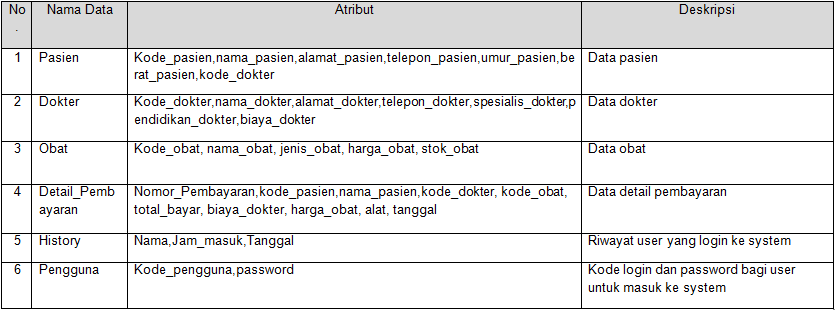
\includegraphics[width=13cm]{gambar/KebutuhanData.png} 

Gambar 1. Analisis Kebutuhan Data
\end{center}


\section{Analisa Kebutuhan Proses}
Analisa kebutuhan proses merupakan penentuan proses (kegiatan) yang akan dimunculkan dalam Aplikasi sistem klinik Kasih Ibu sesuai dengan kebutuhan pengguna. Tahapan ini menjadi dasar sebelum masuk ke perancangan model, yakni gambaran konseptual dari sistem yang akan dibuat. Berikut analisa kebutuhan proses yang diperlukan :

\begin{center}
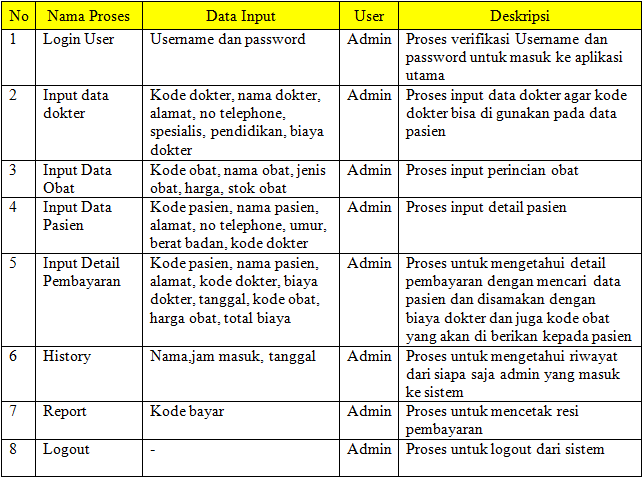
\includegraphics[width=13cm]{gambar/KebutuhanProses.png} 

Gambar 2. Analisis Kebutuhan Proses
\end{center}

\section{Use Case Diagram}
Perancangan awal dibuat ke dalam bentuk diagram use case untuk menjelaskan gambaran sistem dan aktor yang terlibat secara keseluruhan. Komponen use case terdiri dari : Actor, Use Case dan Relation. Aktor adalah user yang berhubungan dengan sistem, yakni admin.

\begin{center}
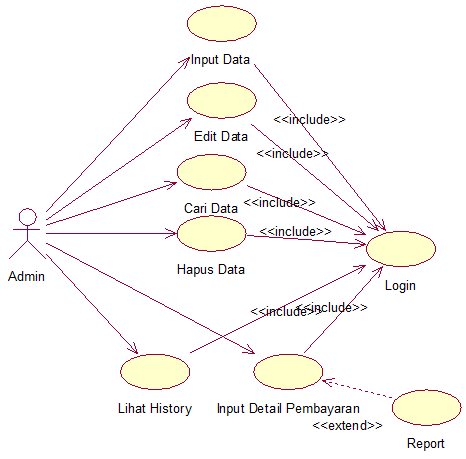
\includegraphics[width=10cm]{gambar/UseCase.png}

Gambar 3. Use Case Diagram
\end{center}

Use case diagram di atas menjelaskan adanya hubungan antara user dengan sistem.


\section{Class Diagram Class}
Diagram membantu kita dalam visualisasi struktur kelas-kelas dari suatu sistem dan merupakan tipe diagram yang paling banyak dipakai. Class diagram memperlihatkan hubungan antar kelas dan penjelasan detail tiap-tiap kelas didalam model desain (dalam logical view) dari suatu sistem. 

Selama proses analisa, class diagram memperlihatkan aturan-aturan dan tanggung jawab entitas yang menentukan perilaku sistem. Selama tahap desain, class diagram berperan dalam menangkap struktur dari semua kelas yang membentuk arsitektur yang dibuat. Class diagram Aplikasi Klinik Kasih Ibu adalah sebagai berikut :

\begin{center}
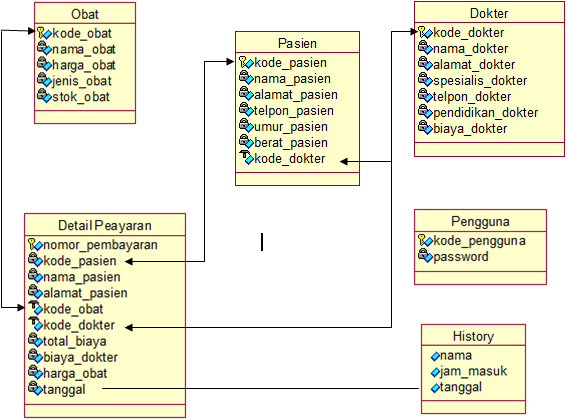
\includegraphics[width=12cm]{gambar/ClassDiagram.png} 

Gambar 4. Class Diagram Class
\end{center}

\section{Jadwal Kegiatan}
Rincian rencana jadwal penelitian dicantumkan dalam tabel berikut.

3.2 Tabel Jadwal Kegiatan Penelitian

\begin{center}
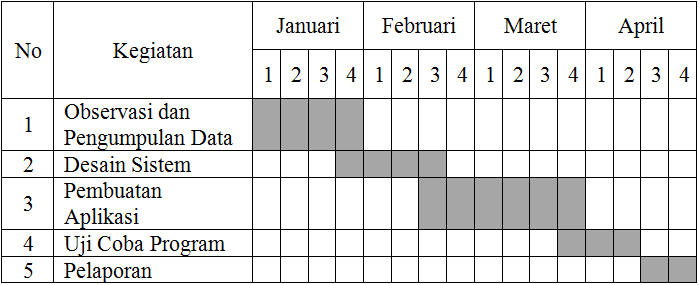
\includegraphics[width=13cm]{gambar/jadwal.png} 
\end{center}




%-----------------------------------------------------------------
%Disini akhir masukan Bab
%-----------------------------------------------------------------

%-----------------------------------------------------------------
%Disini awal masukan untuk Daftar Pustaka
%-----------------------------------------------------------------
%%\nocite{Abel2010,Guerbas201350}
%%\bibliography{research-plan}
%%\bibliographystyle{plainnat}
\begin{thebibliography}{9}

\bibitem[satu(2013)]{satu01}
Raymond McLeod, 1998. Sistem Informasi Managemen Jilid 1 edisi ke tujuh, edisi Bahasa Indonesia, Prentice-Hall

\bibitem[dua(2015)]{dua02}
Amsyah, Zulkifli. 1997. Manajemen Sistem Informasi. Gramedia Pustaka Utama.

\bibitem[tiga(2015)]{tiga03}
Sugiono. 2009. Belajar Oracle dari Nol. Gramedia.


\end{thebibliography}
\addcontentsline{toc}{chapter}{DAFTAR PUSTAKA}
%-----------------------------------------------------------------
%Disini akhir masukan Daftar Pustaka
%-----------------------------------------------------------------

\end{document}